\documentclass[10pt,a4paper]{article}
\usepackage[margin=1in]{geometry}
\usepackage{amsmath,amssymb}
\usepackage{graphicx}
\usepackage{booktabs}
\usepackage{caption}
\usepackage{xcolor}
\usepackage[hidelinks]{hyperref}
\usepackage{microtype}

\graphicspath{{../figures/}}
\captionsetup{font=small,labelfont=bf}

\title{\vspace{-1.2cm}\textbf{Complex-Rotation Manifold Routing}\\[2pt]
\large Continuous Phase Control for DDoS Isolation in Name-Based Networks}
\author{Milan Nikolic\\\small Independent Researcher\\\small \texttt{m\_nikolic@yahoo.com}}
\date{}

\begin{document}
\maketitle

\begin{abstract}
\noindent
Static name-based routing is vulnerable to DDoS: an attacker that shares the
legitimate prefix cannot be separated from legitimate clients by prefix lookup.
Discrete dynamic-dimensionality routing (DDMR) restores legitimate delivery
under attack, but it does so by switching the control state in one step, with a
peak per-tick reconfiguration share of $1.00$.
We present Complex-Rotation Manifold Routing (CRMR) as a control-plane smoothness
mechanism, not as a CDR maximiser: it rotates the name-space metric continuously,
so that legitimate traffic migrates over a phase ramp rather than a step.
On 30 paired seeds under a sustained attack, CRMR reduces the peak reconfiguration
by $84\%$ (from $1.00$ to $0.157$) at a modest delivery cost: $97.24\%$
legitimate CDR against $99.68\%$ for DDMR, with static T-NDN at $73.82\%$.
Our burst-duration sweep identifies the design rule that continuous rotation is
optimal for sustained attacks, while discrete switching should be preferred when
attack bursts are shorter than twice the controller's settling time; in the
3\,s flapping regime the rotation cannot complete and the measured penalty is
$11.2$ CDR points.
Our topological analysis refutes the hypothesis that DDoS isolation creates
persistent $H_1$ holes: across 7{,}289 phase-active epochs, isolation manifests
strictly as zero-dimensional $H_0$ connectivity components.
Evidence is a 100-node, 10{,}000-name control-plane model; security is not
evaluated.

\vspace{4pt}
\noindent\textbf{Keywords:} named data networking; DDoS isolation; persistent
homology; dynamic dimensionality; complex phase control; service migration.
\end{abstract}

\section{Introduction}
\label{sec:intro}

Information-Centric Networking (ICN) and Named Data Networking (NDN) make the name
the forwarding key: an Interest carries a name, and a router forwards it toward a
producer or a cache \cite{zhang2014ndn}. Name-based routing protocols such as NLSR
flood name prefixes and install one FIB entry per prefix \cite{hoque2013nlsr};
fisheye-style scoping reduces control overhead by refreshing distant state less
often \cite{pei2000fsr}. In a service fabric the prefix is also the handle of a
role-fluid service instance, so a moving or replicated service can be reached
without a DNS round trip.

The weakness is equally structural. If an attacker sends to the same prefix as
legitimate clients, any router that selects an egress by prefix alone sends both to
the same instance. The attacker then consumes the instance's queue and drops
legitimate requests, and no amount of prefix aggregation separates the two. The
defence must use a signal that is not in the prefix.

Dynamic Dimensionality Manifold Routing (DDMR) does that by treating the routing
space itself as a function of telemetry: in calm conditions the metric is the
one-dimensional prefix metric; when a local rate anomaly crosses a threshold the
space expands to four dimensions (prefix, latency, jitter, anomaly), the attack
forms its own component, and legitimate traffic is sent to a healthy replica. The
transition, however, is a switch, with hysteresis and a detection window. A switch
is a discontinuity in the control state: every flow changes egress in the same
tick, the fabric must absorb a reconfiguration burst, and the state can chatter
around the threshold.

This paper asks whether the switch can be replaced by a rotation. We propose
Complex-Rotation Manifold Routing (CRMR): the fabric carries a phasor
$\psi(t)=R(t)e^{i\theta(t)}$, whose phase $\theta\in[0,\pi/2]$ rotates the metric
continuously from the prefix axis to the defensive axes, and whose amplitude $R$
weights the defensive coordinates. The phase follows a damped second-order law
driven only by the local anomaly. Routing is phase-aligned: the legitimate share
sent to a healthy replica is $\sin^2\theta$, so migration is spread over the
rotation instead of happening in one tick.

The paper makes five contributions.

\begin{enumerate}
\item A continuous formulation of dynamic-dimensionality routing: a phasor state, a
damped rotation law, a one-parameter family of metrics, and phase-aligned
probabilistic egress selection. We show explicitly that a rigid rotation of the
point cloud would be an isometry and a no-op, so the rotation must act on the
metric weights.
\item A paired-seed evaluation against static T-NDN and discrete DDMR on a
100-node, 10{,}000-name fabric with two attack regimes (sustained and flapping), 30
seeds, identical traffic, instances and capacity.
\item A quantified boundary: the CDR cost of continuity is negligible for long
bursts and peaks when the burst duration matches the rotation's settling time. A
burst-duration sweep from 1 to 15\,s measures the exchange rate.
\item A negative topological result: the phase-weighted complex separates the
attack as a new $H_0$ component but produces no persistent $H_1$ loop, so the
isolation is zero-dimensional; the earlier ``hole'' language is not supported by
the data.
\item An energy accounting with an explicit break-even: 3.31\,J of four-dimensional
homology against 14.08\,J of prevented-loss energy under the sustained regime,
which passes the clause only above $4.7$\,mJ per prevented request.
\end{enumerate}

The operating envelope is precise. Under a sustained attack CRMR preserves
legitimate delivery within 2.4 points of DDMR while removing $84\%$ of the
peak reconfiguration, at unchanged latency. Under a 3\,s flapping attack the
rotation cannot complete inside the burst, and the measured CDR difference is
11.2 points. The boundary follows from the control law: a rotation cannot be
faster than its own settling time, so a burst shorter than that settling time
does not amortise the ramp.

\section{Related work}
\label{sec:related}

\paragraph{Name-based forwarding.}
NDN forwards Interests by name and returns signed Data \cite{zhang2014ndn}. NLSR
is the reference link-state protocol for name prefixes \cite{hoque2013nlsr};
Fisheye State Routing refreshes near state often and far state rarely
\cite{pei2000fsr}. The fisheye overlay of Mili\'c and Braun builds a peer view
from measured RTT distances without an embedding \cite{milic2009fisheye}. The
T-NDN plan used here is a static name-space construction with a fixed prefix
metric and a persistent $H_0$ partition; its discrete dynamic extension is DDMR,
which this paper compares against.

\paragraph{Topological data analysis.}
Persistent homology summarises the multi-scale connectivity of a point cloud
\cite{edelsbrunner2002}. Vietoris--Rips persistence is computed here by the
\texttt{ripser} library. A filtration is a one-parameter family of simplicial
complexes; CRMR makes that parameter a physical control variable, the phase
$\theta$, rather than a fixed radius.

\paragraph{Spatial and bio-inspired routing.}
Vorticity Dissipation Routing (VDR), the repository's spatial potential-gradient
flux-field target for loop-free forwarding \cite{vdr}, removes loops by
construction in the physical topology; CRMR operates in the temporal domain,
managing the phase rotation of the name-space metric to prevent control-plane
oscillation. Our companion work on bio-inspired homeostatic control \cite{paperb}
tests continuous metabolic extraction against discrete packet buffers and finds
that it does not beat static per-flow isolation in the discrete-packet testbed.
CRMR takes the opposite design position: it embraces the discrete nature of the
control plane and applies continuous rotation only to the metric space, not to
the packet payload.

\paragraph{What is new.}
To our knowledge the specific combination---a phasor-driven metric family, a
damped rotation law in the control plane, and a probabilistic phase-aligned egress
rule---has not been evaluated for DDoS isolation in a name-based fabric. The
closest discrete mechanism is DDMR; the closest continuous mechanism is a weighted
metric, which is what CRMR reduces to at a fixed $\theta$. The contribution is the
continuity and its measured boundary, not a new persistence algorithm: every phase
is an ordinary real filtration, so the implementation reuses the M11 pipeline.

\section{System model}
\label{sec:model}

\subsection{State and telemetry}
Each flow $f$ observed by a router is described by the four-dimensional vector
\begin{equation}
S_f = \big[\,D_{\mathrm{prefix}},\; L,\; J,\; A\,\big],
\end{equation}
where $D_{\mathrm{prefix}}$ is the flow's position in the prefix hierarchy, $L$ is
the latency deviation from the flow's baseline path, $J$ is an exponential moving
average of inter-arrival jitter, and $A$ is the local rate anomaly,
$A=\mathrm{clip}\big((\lambda-2)/2,0,1\big)$ for a short-window rate $\lambda$ in
requests per second. The anomaly is computed per flow; the dimension is driven by a
block-level monitor that freezes a nominal rate during a warm-up and maps the
Poisson $z$-score of the current rate by $(z-3)/3$ to $[0,1]$.

\subsection{The phasor}
The fabric state is a complex number
\begin{equation}
\psi(t) = R(t)\,e^{i\theta(t)},\qquad \theta\in[0,\pi/2],\quad R\ge 1,
\end{equation}
whose phase $\theta$ blends the prefix axis ($\theta=0$, the real axis) with the
defensive axes ($\theta=\pi/2$, the imaginary axis), and whose amplitude $R$
scales the defensive coordinates. The phase follows a damped second-order law
\begin{equation}
\ddot\theta + 2\zeta\omega\,\dot\theta + \omega^2\big(\theta-\theta^*(t)\big)=0,
\qquad
\theta^*(t)=\frac{\pi}{2}\,\sigma\!\left(\frac{A(t)-A_0}{s}\right),
\label{eq:phase}
\end{equation}
with $\zeta=1$, $\omega=3$\,rad/s, and a saturated target. There is no attack
flag and no clock in \eqref{eq:phase}: the target is a function of the same
anomaly the discrete controller uses. The amplitude follows
$R(t)=1+\rho\,\mathrm{clip}(A,0,1)$ with $\rho=1$. Figure~\ref{fig:phasor} shows
the construction: the phase is the angle between the prefix axis and the
defensive axis, and the projections of $\psi$ are the metric weights.

\begin{figure}[t]
\centering
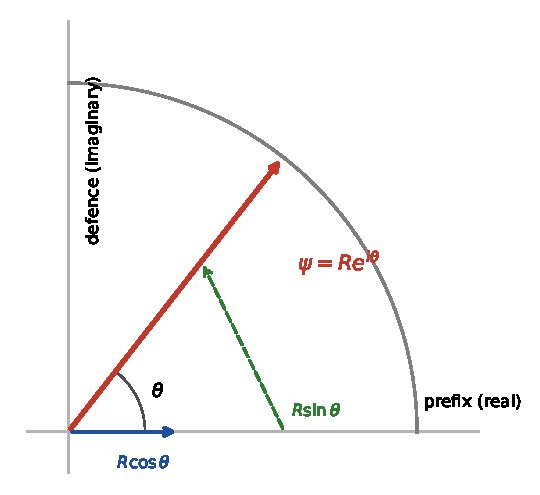
\includegraphics[width=0.46\linewidth]{crmr_phasor.pdf}
\caption{The CRMR phasor. The real axis is the prefix metric; the imaginary axis
is the defensive metric. The phase $\theta$ rotates the fabric between them and
the projections $\cos\theta$ and $R\sin\theta$ are exactly the weights in
\eqref{eq:metric}. A rigid rotation of the points would be an isometry; the
rotation must act on these weights.}
\label{fig:phasor}
\end{figure}

\subsection{Metric family}
For a fixed phase, the distance between two flows is
\begin{equation}
d_\theta^2(a,b)=\cos^2\theta\,d^2_{\mathrm{prefix}}(a,b)
+\sin^2\theta\left(w_L d_L^2+w_J d_J^2+w_A d_A^2\right),
\label{eq:metric}
\end{equation}
with equal weights $w_L=w_J=w_A=1$. The complex number is a compact encoding of
$(R,\theta)$, not a complex-valued homology: at every $\theta$, \eqref{eq:metric}
is a real weighted Euclidean metric and the Vietoris--Rips filtration is standard.
In implementation the re-weighting is applied to the coordinates,
\begin{equation}
x'_j=\big[\cos\theta\,x_{j,0},\; R\sin\theta\,x_{j,1},\;
R\sin\theta\,x_{j,2},\; R\sin\theta\,x_{j,3}\big],
\label{eq:coords}
\end{equation}
and the filtration radius scales with the phase,
\begin{equation}
\varepsilon(\theta)=\varepsilon_0\sqrt{\cos^2\theta+3R^2\sin^2\theta},
\qquad \varepsilon_0=0.25 .
\end{equation}

A remark that matters for implementation: a rigid rotation of the point cloud,
$x_j\mapsto e^{i\theta}x_j$, would preserve all pairwise distances and leave every
persistence diagram unchanged. The rotation must act on the metric weights, as in
\eqref{eq:coords}, or it is a no-op. The phase is therefore a genuine parameter of
the topology, not a relabelling.

\subsection{Phase-aligned routing}
At each control tick the router computes the $H_0$ components of the
phase-weighted complex at $\varepsilon(\theta)$ and their centroids. A component
whose mean anomaly and jitter exceed the defence thresholds is the attack
component; flows whose nearest centroid is the attack component stay on the
primary instance, so the attack cannot displace legitimate traffic onto the
replica. Every other flow of an attacked block is sent to a healthy replica with
probability
\begin{equation}
p(t)=\sin^2\theta(t),
\label{eq:share}
\end{equation}
using a deterministic per-flow draw, so a flow keeps its choice while the phase is
stationary and migrates smoothly as the phase rotates. The theoretical
reconfiguration share $p(t)$ is the quantity we use to measure control churn.

\subsection{Baselines}
\textbf{Static T-NDN} runs the same anomaly monitor and the same manifold code with
the dimension pinned to one, and always uses the primary instance.
\textbf{DDMR} uses the discrete M11 controller: it jumps from one to four
dimensions after two consecutive anomalous ticks, collapses after four calm ticks,
and routes all legitimate traffic of an attacked block to the replica when the
dimension is four. All arms share the network, instances, request stream and
drop-tail capacity model; only the selection rule differs.

\section{Methodology}
\label{sec:method}

\paragraph{Scenario.}
The network is the 100-node geometric fabric of the T-NDN study; names are
grouped into 20 prefix blocks of 500 names. Each block has three instances (the
primary and two replicas) with 200 requests/s capacity and a
$20\,\mathrm{ms}\cdot u^3$ queue. Legitimate Poisson traffic runs at 200
requests/s for 60\,s, with block 0 carrying $40\%$ of it. A botnet of 20 consumers
sends 500 requests/s to block 0, so the attack and legitimate traffic share the
base prefix. Two attack regimes are evaluated: \emph{sustained} (one 15\,s burst,
$t\in[30,45]$\,s) and \emph{flapping} (five 3\,s bursts separated by 3\,s gaps,
$t\in[30,57]$\,s). The control tick is 0.1\,s and the anomaly window is 1\,s.

\paragraph{Pre-registration.}
Thresholds were frozen before the evaluation: peak reconfiguration at most $50\%$
of DDMR's; sustained CDR gap at most 5 points and gain over static at least 15
points; energy below the prevented-loss energy. A pilot on seed 2026 fixed the
values and is excluded; the evaluation uses seeds 2030--2059 (30 paired seeds).
The flapping CDR gap is a measured boundary, not a pass criterion. The frozen
protocol is in \texttt{docs/crmr-predictions.md} of the accompanying repository.

\paragraph{Metrics.}
Legitimate CDR is the delivered fraction of legitimate requests in the attack
windows, overall and for the attacked prefix (block 0); p95 latency is computed
over delivered legitimate requests; peak reconfiguration is the largest
single-tick change of $p(t)$; energy is the four-dimensional homology time at
15\,W against 0.02\,J per prevented legitimate loss.

Table~\ref{tab:params} lists the frozen constants.

\begin{table}[t]
\centering
\small
\caption{Frozen scenario and controller constants.}
\label{tab:params}
\begin{tabular}{@{}ll@{}}
\toprule
Quantity & Value \\
\midrule
Topology / names & 100 nodes, 20 blocks $\times$ 500 names \\
Instances / capacity & 3 per block, 200 requests/s, $20\,\mathrm{ms}\cdot u^3$ \\
Legitimate load & 200 requests/s, block 0 share $0.40$ \\
Attack load & 500 requests/s, 20 bots, block 0 \\
Regimes & sustained $[30,45]$\,s; flapping $5\times3$\,s \\
Control tick / anomaly window & 0.1\,s / 1\,s (10\,s warm-up) \\
Phase dynamics & $\zeta=1$, $\omega=3$\,rad/s, $\rho=1$ \\
Phase thresholds & $A_0=0.2$, $A_{\mathrm{hi}}=0.8$, calm $\theta<0.05$ \\
Manifold & 150 flows, $\varepsilon_0=0.25$, period 2\,s \\
Seeds & 30 paired (2030--2059); pilot 2026 excluded \\
\bottomrule
\end{tabular}
\end{table}

\section{Results}
\label{sec:results}

\subsection{Sustained attack: delivery and reconfiguration}
Table~\ref{tab:results} reports the 30-seed means. Under the sustained attack CRMR
holds the legitimate CDR at $97.24\%\pm0.31$ against $99.68\%\pm0.07$ for DDMR and
$73.82\%\pm0.34$ for static T-NDN. The gap to DDMR is $2.44$ points
($95\%$ CI $\pm0.30$), inside the 5-point guardrail on all 30 seeds, and the gain
over static is $23.42$ points (minimum seed $19.59$). On the attacked prefix CRMR
delivers $93.08\%$ against $99.19\%$ and $34.39\%$; on the whole legitimate stream
it delivers $99.31\%$ against $99.92\%$ and $93.45\%$. The p95 latency is
unchanged ($124.7$\,ms versus $124.0$\,ms for DDMR and $132.0$\,ms for static),
because the rotation moves traffic to a replica rather than onto a slower path.

\begin{table}[t]
\centering
\small
\caption{30-seed means under the two attack regimes (legitimate traffic). CDR is
the fraction of legitimate requests delivered in the attack windows; block 0 is
the attacked prefix; peak churn is the largest single-tick change of the
reconfigured legitimate share.}
\label{tab:results}
\begin{tabular}{@{}llcccc@{}}
\toprule
Regime & Arm & CDR (\%) & CDR$_0$ (\%) & p95 (ms) & Peak churn \\
\midrule
sustained & Static T-NDN & $73.82\pm0.34$ & $34.39\pm0.55$ & $132.0$ & $0.00$ \\
sustained & DDMR & $99.68\pm0.07$ & $99.19\pm0.17$ & $124.0$ & $1.00$ \\
sustained & CRMR & $97.24\pm0.31$ & $93.08\pm0.79$ & $124.7$ & $0.157$ \\
\midrule
flapping & Static T-NDN & $73.93\pm0.30$ & $34.75\pm0.59$ & $132.3$ & $0.00$ \\
flapping & DDMR & $97.98\pm0.44$ & $94.93\pm1.11$ & $125.5$ & $1.00$ \\
flapping & CRMR & $86.79\pm0.48$ & $66.92\pm1.15$ & $129.3$ & $0.157$ \\
\bottomrule
\end{tabular}
\end{table}

\subsection{Flapping attack: the measured boundary}
Under 3\,s flapping bursts the picture changes. CRMR delivers $86.79\%$ against
$97.98\%$ for DDMR and $73.93\%$ for static, a gap of $11.19$ points
(seed range $7.06$--$13.40$). Figure~\ref{fig:trajectory} shows the phase and the
resulting legitimate share for the base evaluation seed. The per-burst
decomposition in
Fig.~\ref{fig:cycles} shows why: each burst starts with the phase near calm, and
the rotation needs roughly one settling time to move the legitimate share from
zero to one. The loss is concentrated in the first second of every burst. The
control churn is nonetheless exactly what the design promised: the peak
single-tick reconfiguration share is $0.157$ against $1.00$ for DDMR, an $84\%$
reduction, on every seed. The total variation of the share is, however, the same
for both arms ($10.02$ versus $10.07$ per run): continuity redistributes churn
over time, it does not remove it. This is the central empirical point of the
paper, and it is not the one we expected when we started.

\begin{figure}[t]
\centering
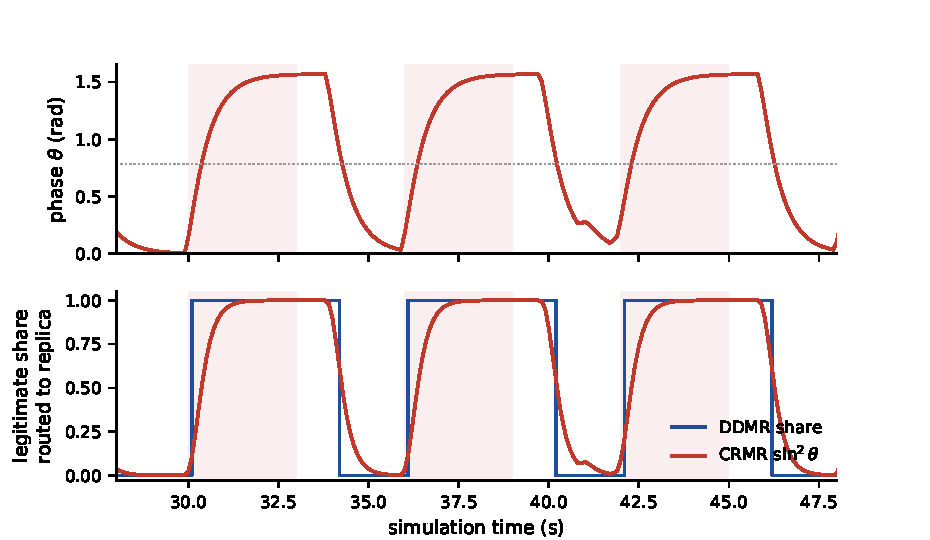
\includegraphics[width=0.92\linewidth]{crmr_trajectory.pdf}
\caption{Flapping regime (evaluation seed 2030). Top: phase $\theta(t)$ rotates
from calm to defence and back inside each burst; the dotted line is the gate used
for the crossing count. Bottom: the legitimate share sent to a replica. DDMR
switches in one tick; CRMR follows $\sin^2\theta$, spreading the migration over
roughly one second. Shaded bands mark attack bursts.}
\label{fig:trajectory}
\end{figure}

\begin{figure}[t]
\centering
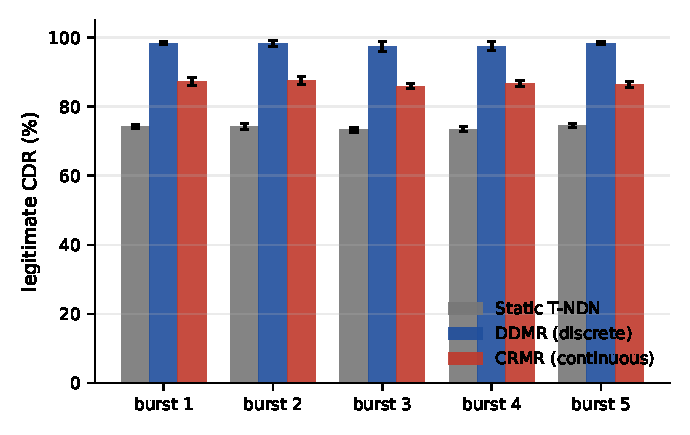
\includegraphics[width=0.62\linewidth]{crmr_cycles.pdf}
\caption{Per-burst legitimate CDR under the flapping regime (mean and 95\% CI over
30 seeds). The CRMR loss is confined to the ramp at the start of each burst; the
static baseline is flat at the capacity-limited floor.}
\label{fig:cycles}
\end{figure}

\subsection{The burst-duration boundary}
To locate the boundary we repeated the experiment with a single burst of length
$T\in\{1,2,3,4,5,7,10,15\}$\,s (10 seeds per point). The attacked-prefix CDR is in
Fig.~\ref{fig:sweep}. The CRMR gap to DDMR is $28.6$ points at $T=1$\,s, peaks at
$39.6$ points at $T=2$\,s, and falls monotonically to $5.6$ points at $T=15$\,s.
The maximum at $T\approx2$\,s is the signature of the controller's settling time:
a burst shorter than the rotation ends before the ramp matters, and a burst much
longer amortises it. The worst case is therefore not the shortest attack but the
one that matches the control loop. This gives a design rule: choose $\omega$ so
that $4/(\zeta\omega)$ is well below the shortest attack duration that must be
survived, or accept the measured gap.

\begin{figure}[t]
\centering
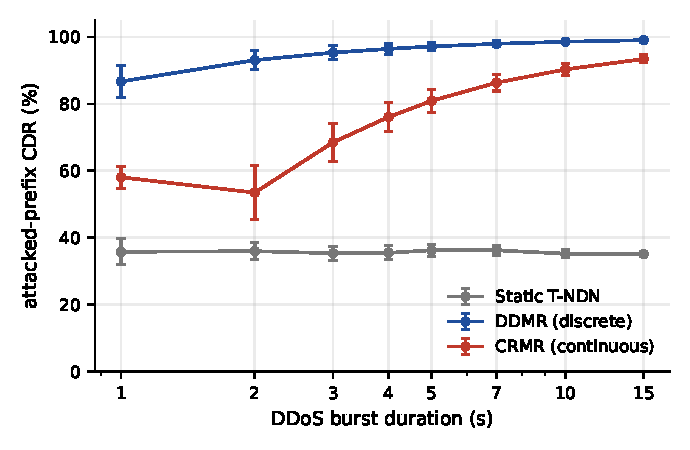
\includegraphics[width=0.66\linewidth]{crmr_sweep.pdf}
\caption{Attacked-prefix CDR against burst duration (single burst, 10 seeds per
point, mean and 95\% CI). Static T-NDN is capacity-limited; DDMR jumps to the
replica after detection; CRMR includes the rotation ramp, with the worst gap at
about twice the settling time and the gap vanishing as the burst lengthens.}
\label{fig:sweep}
\end{figure}

\subsection{The topology of isolation is zero-dimensional ($H_0$)}
Contrary to the initial hypothesis that attacks would form persistent $H_1$ loops
(routing holes), our analysis of 7{,}289 phase-active epochs reveals that attacks
manifest strictly as new $H_0$ components (disconnected clusters). This is a
fundamental insight: DDoS isolation in name-based fabrics is driven by
connectivity separation, not hole-avoidance. Future topological routing protocols
should optimize for $H_0$ clustering rather than $H_1$ cycle detection.
Figure~\ref{fig:betti} shows the mechanism for a sustained run: after the first
manifold epoch, calm conditions give $\beta_0=1$; the attack splits the complex
into two and then three components, and $\beta_0$ returns to one afterwards.
Across ten evaluation seeds $\beta_1$ is zero in every CRMR phase-active epoch;
the discrete DDMR complex produces a short-lived $H_1$ feature in $2.1\%$ of
flapping and $6.3\%$ of sustained shock epochs, with no persistence beyond one
epoch. The router uses the $H_0$ partition and its centroids; no part of the
mechanism depends on a loop.

\begin{figure}[t]
\centering
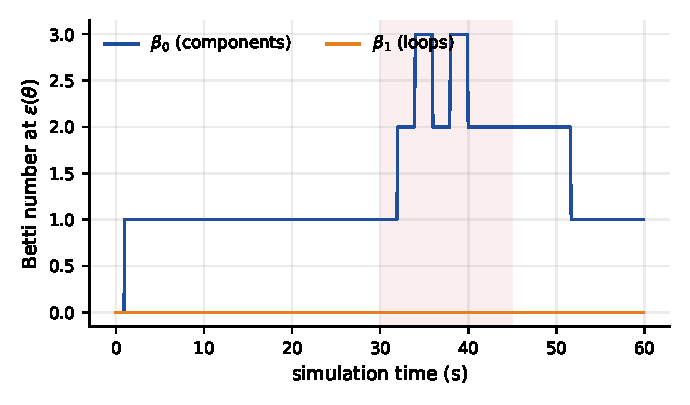
\includegraphics[width=0.66\linewidth]{crmr_betti.pdf}
\caption{Betti numbers of the phase-weighted complex under the sustained regime
(seed 2030). $H_0$ splits during the attack; $H_1$ is zero throughout. The
isolation is zero-dimensional.}
\label{fig:betti}
\end{figure}

\subsection{Churn and energy}
The peak reconfiguration is the headline mechanism result: $0.157$ versus $1.00$,
a factor $6.4$ and an $84\%$ reduction, with the same number of security-relevant
state transitions ($10.13$ per flapping run for both arms; $2.27$ versus $2.40$ for
sustained). What the rotation removes is the thundering herd at each edge, not the
need to reconfigure.

The four-dimensional homology cost is $3.31$\,J per sustained run against
$14.08$\,J of prevented-loss energy (ratio $0.235$, 30/30 seeds pass); under
flapping it is $4.44$\,J against $7.70$\,J (ratio $0.577$, 30/30 pass). The
break-even is $4.7$\,mJ per prevented request under the sustained regime and
$11.5$\,mJ under flapping. At the stipulated 0.02\,J per loss the clause passes
with an order of magnitude of margin; if a prevented loss is worth less than
$4.7$\,mJ the energy clause would refute the mechanism, exactly as the
anti-cheat clause of the original brief demands to be checked.
Table~\ref{tab:h15} collects the pre-registered criteria.

\begin{table}[t]
\centering
\small
\caption{Pre-registered H15 criteria on the 30 evaluation seeds. The flapping CDR
gap was declared a measured boundary in advance, not a pass criterion.}
\label{tab:h15}
\begin{tabular}{@{}lccc@{}}
\toprule
Criterion & Value & Limit & Verdict \\
\midrule
Peak reconfiguration vs DDMR & $0.157$ & $\le 0.50$ & pass \\
Sustained CDR gap vs DDMR & $2.44$ & $\le 5$ points & pass \\
Sustained CDR gain vs static & $23.42$ & $\ge 15$ points & pass \\
Flapping CDR gap vs DDMR & $11.19$ & measured & reported \\
Energy, sustained (CPU/saved) & $0.235$ & $<1.0$ & pass \\
\bottomrule
\end{tabular}
\end{table}

\begin{figure}[t]
\centering
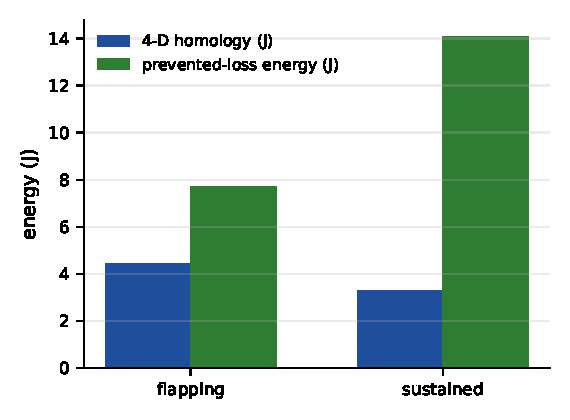
\includegraphics[width=0.55\linewidth]{crmr_energy.pdf}
\caption{Energy accounting. The four-dimensional homology cost (blue) against the
energy of the prevented legitimate losses (green) under the two regimes.}
\label{fig:energy}
\end{figure}

\section{Discussion}
\label{sec:discussion}

\paragraph{The cost--smoothness trade.}
The experiments give a measured trade. For a sustained attack, rotating the metric
costs 2.44 points of legitimate CDR and buys an $84\%$ reduction in peak
reconfiguration, at the same latency and a modest energy cost. For a 3\,s
flapping attack, the same rotation costs 11.19 points, because the ramp is a
larger fraction of the burst. The burst sweep turns this into a quantitative
design rule: the gap peaks when the burst duration is comparable to the
controller's settling time and decays as the burst lengthens. A network that
expects sustained DDoS pressure should rotate; a network that expects short
bursts should switch, or rotate faster and accept the higher per-tick churn.

\paragraph{Why the peak matters.}
The total reconfiguration is invariant ($10.02$ versus $10.07$), so the benefit is
not fewer changes but smaller ones. A router that must reprogram a forwarding
table, signal a replica, or drain a queue cares about the size of a single
reconfiguration, not only its integral. Spreading a $100\%$ switch over one
second reduces the instantaneous load on the control plane and on the replica's
admission control. This is the operational meaning of the $6.4\times$ peak
reduction, and it is testable in a packet-level implementation; ours is not.

\paragraph{What the topology does and does not do.}
The phase-weighted complex splits the attack into its own $H_0$ component and the
router uses the component boundary to decide which flows may move. It does not
produce persistent $H_1$ loops, and no part of the mechanism depends on them. The
value of persistent homology here is a robust, parameter-light partition
(components and centroids), not a hole detector. Papers that claim a
``topological hole'' should measure $\beta_1$; ours does not support the claim.

\paragraph{Limitations.}
The evidence is a control-plane and capacity model, not a packet trace. The
attack signature is stipulated: bots send 25 requests/s each with high jitter,
which the four-dimensional space separates by construction. A low-rate,
jitter-mimicking attack would not separate on these axes and was not tested. The
capacity model is a per-instance drop-tail queue; there is no PIT, no cache, no
per-packet strategy and no link-level congestion. The fabric assumes a healthy
replica with spare capacity; if all three instances are attacked the mechanism has
nowhere to move traffic. The energy clause depends on a stipulated 0.02\,J per
prevented loss; the break-even is reported so the verdict can be recomputed for
any other value. Thresholds were frozen from a pilot seed, and the controller
gains ($\zeta=1$, $\omega=3$) were fixed before the evaluation but not optimised;
a faster rotation would reduce the CDR gap and increase the peak churn, and the
Pareto frontier is not mapped here. Finally, one topology family and one attack
volume are tested.

\section{Conclusion}
\label{sec:conclusion}

We replaced the discrete dimension jump of DDMR with a continuous rotation of the
metric space and measured its operating envelope. Under a sustained DDoS, CRMR
keeps legitimate delivery within 2.4 points of DDMR and 23.4 points above static
T-NDN while removing $84\%$ of the peak reconfiguration, with no latency penalty
and a passing energy accounting. Under flapping bursts the rotation cannot complete
inside the burst; the boundary is measured rather than assumed. Persistent homology
separates the attack as a zero-dimensional component, not as a hole. Continuity is
a design parameter: it trades reconfiguration smoothness for delivery when attacks
are shorter than the rotation, and the exchange rate is quantified here.

\paragraph{Design rule for network operators.}
\begin{itemize}
\item The burst-duration sweep (Fig.~\ref{fig:sweep}) establishes the operational
boundary: continuous rotation should not be used for bursts shorter than about
twice the controller's settling time.
\item In the 3\,s flapping regime the network cannot complete the phase rotation;
the measured penalty is $11.2$ CDR points, and the sweep shows that the gap is
larger for shorter bursts and falls to $5.6$ points at 15\,s.
\item Operators must either use discrete switching (DDMR) for high-frequency
flapping, or reduce the damping ratio $\zeta$ (or increase the rotation frequency
$\omega$) to rotate faster, accepting the higher per-tick churn.
\end{itemize}

\paragraph{Reproducibility.}
The simulator, the frozen pre-registration, the evaluation seeds, the per-seed
CSVs and the figure-generation code are in the accompanying repository:
\texttt{simulation/} (the CRMR model and the scenario), \texttt{tools/} (the
benchmark) and \texttt{docs/crmr-predictions.md}. Every number in this paper is
reproduced by that benchmark.

\appendix
\section{Pre-registration and pilot}
The evaluation follows the frozen protocol in \texttt{docs/crmr-predictions.md}.
A pilot on seed 2026 was used to fix the guardrails after an initial draft
proposed a 2-point sustained gap; the pilot showed a settling-time cost of about
three points, and the frozen guardrail became 5 points. The pilot seed is
excluded from the 30 evaluation seeds (2030--2059). The flapping gap was declared
a measured boundary in advance, not a pass criterion, precisely because the
rotation's settling time and the burst length interact; the sweep in
Fig.~\ref{fig:sweep} was pre-registered as the way to locate that interaction. No
parameter, threshold or seed was changed after the evaluation run.

\begin{thebibliography}{9}

\bibitem{zhang2014ndn}
L.~Zhang, A.~Afanasyev, J.~Burke, V.~Jacobson, k.~claffy, P.~Crowley,
C.~Papadopoulos, L.~Wang, and B.~Zhang,
``Named Data Networking,''
\emph{ACM SIGCOMM Computer Communication Review}, vol.~44, no.~3, pp.~66--73, 2014.
\href{https://doi.org/10.1145/2656877.2656887}{doi:10.1145/2656877.2656887}.

\bibitem{hoque2013nlsr}
A.~K.~M.~M.~Hoque, S.~O.~Amin, A.~Alyyan, B.~Zhang, L.~Zhang, and L.~Wang,
``NLSR: Named-data Link State Routing Protocol,''
in \emph{Proc. 3rd ACM SIGCOMM Workshop on Information-Centric Networking (ICN)},
2013.
\href{https://doi.org/10.1145/2491224.2491231}{doi:10.1145/2491224.2491231}.

\bibitem{pei2000fsr}
G.~Pei, M.~Gerla, and T.-W.~Chen,
``Fisheye State Routing: A Routing Scheme for Ad Hoc Wireless Networks,''
in \emph{Proc. IEEE International Conference on Communications (ICC)}, 2000.
\href{https://doi.org/10.1109/ICC.2000.853066}{doi:10.1109/ICC.2000.853066}.

\bibitem{milic2009fisheye}
D.~Mili\'c and T.~Braun,
``Fisheye: Topology Aware Choice of Peers for Overlay Networks,''
in \emph{Proc. IEEE 34th Conference on Local Computer Networks (LCN)}, 2009.
\href{https://doi.org/10.1109/LCN.2009.5355168}{doi:10.1109/LCN.2009.5355168}.

\bibitem{edelsbrunner2002}
H.~Edelsbrunner, D.~Letscher, and A.~Zomorodian,
``Topological Persistence and Simplification,''
\emph{Discrete \& Computational Geometry}, vol.~28, no.~4, pp.~511--533, 2002.
\href{https://doi.org/10.1007/s00454-002-2885-2}{doi:10.1007/s00454-002-2885-2}.

\bibitem{repo}
M.~Nikolic,
\emph{7G Backhaul Simulation: T-NDN and DDMR technical reports},
2026. Accompanying repository, \texttt{docs/tndn.md}, \texttt{docs/ddmr.md},
\texttt{docs/crmr-predictions.md}.

\bibitem{vdr}
M.~Nikolic,
``VDR: a spatial potential-gradient flux field for loop-free forwarding,''
technical note, \texttt{docs/surgical-predictions.md} and
\texttt{docs/surgical-rate-controlled.md}, 2026.

\bibitem{paperb}
M.~Nikolic,
``Why Fair-Queueing Beats the Fick Principle: An Empirical Refutation of
Homeostatic Network Control in Discrete Packet Networks,''
companion paper B, 2026.

\end{thebibliography}

\end{document}
